\chapter{Knowledge Graphs for Cell Communications}
\label{06kg}

\section{Introduction}

\begin{figure}
    \centering
    \includegraphics{06kg/figs/6KG_com.png}
    \caption{}
    \label{fig:6intro}
\end{figure}

Cellular signalling involves a complex series of directed and hierarchical~\cite{kumar_3_2003} signal transduction cascades between molecules that dictate a cell's response to extrinsic and intrinsic cues.

In the context of inter-cellular paracrine communication for example, a secreting cell produces a series of ligands that are captured by receptors on a receiving cell. The receiving cell then might engage in an intra-cellular signal transduction cascade orchestrated by \acrshort{ptm}s, such as the MAPK cascade~\cite{zhang_mapk_2002}. These cascades regulate gene expression downstream of active transcription factors. With overlapping pathways, feedback loops, and complex settings with multiple cells engaging in symmetrical or non-symmetrical communications, there is nonetheless a directional causality-driven signalling information flow (Figure \ref{fig:6intro}).

The physical interactions between molecules are often represented as a network of genes, proteins or even \acrshort{ptm}s, described in the manner of a \acrfull{kg}. These network representations have been extensively explored to model both intra- and inter-cellular communications, but to date they are not consistently analysed using methods that leverage the underlying directed and hierarchical nature of signalling processes, often either treating the graph as undirected or analyzing pairwise relationships between feature detection metrics (such as gene expression)~\cite{pratapa_benchmarking_2020, armingol_deciphering_2020}. 
    % Cellular signaling involves overlapping directed \cite{HANCOCK200364} and hierarchical signal transduction cascades between molecules to coordinate targeted behavior \cite{zhang_mapk_2002}.
    % %The physical interactions of molecules are often represented as a network.
    % The resulting network of molecular interactions determines a cell's response under different conditions, drawing interest towards unifying and characterizing varying sources of molecule signaling from distinct scientific experiments. However, methods to represent biological networks and infer gene-gene relationships rarely take into the account the \textit{directionality} and \textit{hierarchical structure} of these gene graphs.

The field of directed cellular interaction databases already presents with some established curated resources like OmniPath~\cite{turei_integrated_2021}, with a growing number of methods attempting to model the communications in a directed manner~\cite{lefebvre_large-scale_2021}, describing cell-cell interactions~\cite{fischer_modeling_2022,yang_sctenifoldxct_2023}, and even data-driven \emph{de novo} generation of signal transduction networks~\cite{hu_cytotalk_2021}.

Knowledge graph embedding tools aim to learn the complex relational information in heterogeneous directed networks and represent it in a lower dimensional space that can be analysed using more common graph signalling processing and general data analysis approaches. Methods like the classical TransE~\cite{bordes_translating_2013} and its derivatives, graph convolutional networks, and hyperbolic embeddings~\cite{chami_hyperbolic_2019}, represent some of different approaches to learn the strcuture of \acrshort{kg}s.

In this chapter I propose a novel approach for assembling gene-gene graphs that capture cellular communications by leveraging \acrshort{kg} embedding approaches. I aim to project single-cell \emph{omic} profiles into the assembled \acrshort{kg}s, thus treating the cells as signals on a gene graph. The resulting signals can then be treated as another single-cell \emph{omic} view of the cells, and used to generate new embeddings or be compared against their gene expression profiles.

        % Gene embedding methods are growing , so are graph signal processing approaches. 
        % Discuss the embedding methods of these graphs:
        % Complexity in terms of structure, directionality and type of interaction. All of this is very important, unlike in undirected knn grpahs ubiquitous to omic analyses.
        % This means that we need some methods able to compute all of this complex relations in multi relation directed graphs  (MultiDiGraph). methods have been developed, transE \cite{bordes_translating_2013}family, graph convolutional networks, and the stuff from he stanford dawn group on  hyperbolic embeddings  \cite{chami_hyperbolic_2019} and general ML approaches applied to non euclidean spaces.
        % Non-euclidean space like hyperbolic spaces argued to be key because graphs with important hierarchical structure [as is biological signalling] is much better capture in a hyperbole than in a plane \cite{bronstein_geometric_2017,nickel_poincare_2017,chamberlain_neural_2017}.[the first one is general Euclidean =bad, the later ones refer to the cocnept of hierarchical graph better on hyperboles than planes].
        % on the other hand, prelim results in collab porject suggest perhaps not as important for bio KG despite the hierarchical nature of signalling networks.



\section{KG Structure}

\begin{figure}
    \centering
    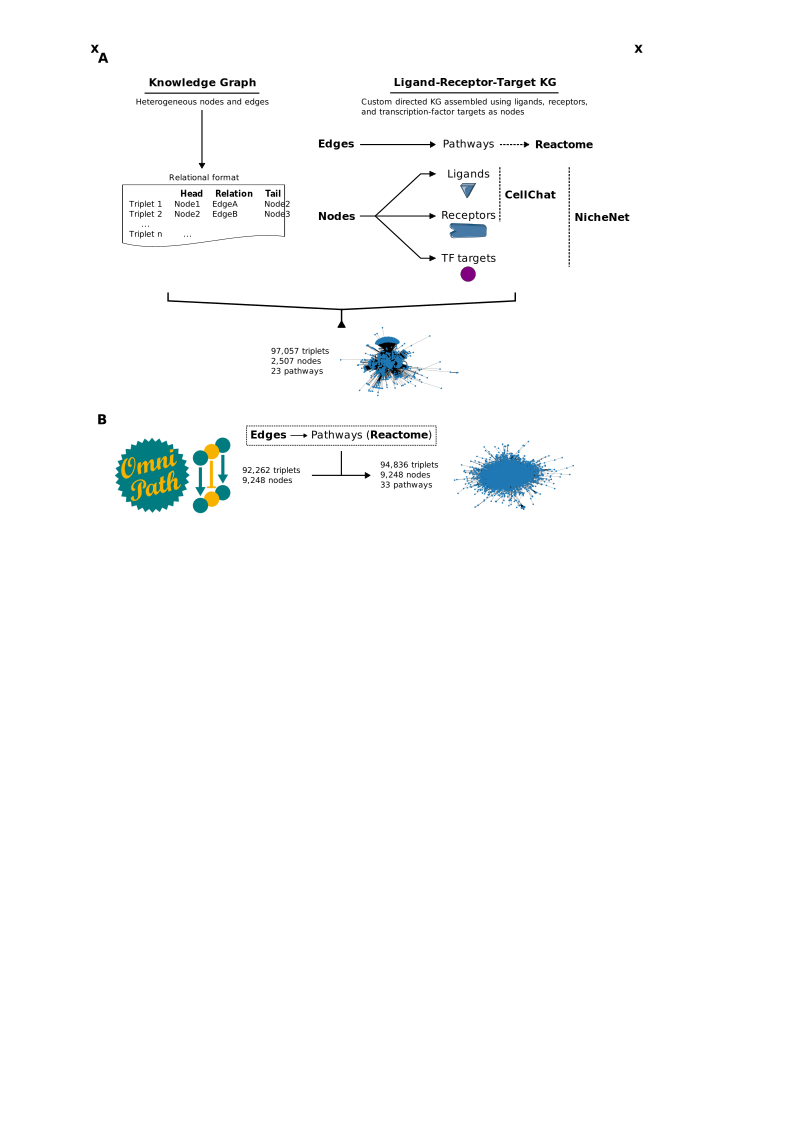
\includegraphics{06kg/figs/6KG_kg.png}
    \caption{}
    \label{fig:6kg}
\end{figure}

Graph assembled from sources, hierarchical directed structure. Nodes are ligands, receptor and gene targets of cellular signalling. Edges established from pathway connecting two nodes. Sources are cellchat and nichenet for nodes and reactome for pathways.

Formatted as head,relation,tail format. Total of XX relations with YY and ZZ nodes.

Compare against common KG such as OmniPath.
Omnipath has a curated functional interactions interaction database comprising genes involved in cellular communications. type of interactions (PTM, ...) consensus, directionality and even logical sense of interaction (activation or repression). HTis datasbase is cureated from public resources.
Process interaction database as before by using OmniPath nodes and edges from reactome pathways. 
Comparable graph in terms of node, but a bit more dense than the LRT KG and with a lower hierarchy score (see Chapter \ref{02methods} for Table \ref{tab:2kg}).



\section{KG Embedding}

\begin{figure}
    \centering
    \includegraphics{06kg/figs/6KG_embed.png}
    \caption{}
    \label{fig:6embed}
\end{figure}

To capture the complex relational information in a simpler format amenable to downstream analyses, .....

Leverage directed nature of graph by embedding on lower space. Methods used (Chapter \ref{02methods}). Exploration of nodes on a DimRed space suggest I can capture topological differences between Ligands , receptors and targets. It also appears that gene targets are the most promiscuous nodes with higher degrees, followed by receptors and finally ligands. However, care must be taken here for three classes are imbalanced.

Biological information is also capture in the KGE, with nodes showing a certain degree of separation by key signalling pathways from REACTOME.
    Looking at nodes thsi means thatwe can see which kind of genes (lignas, receptors, targets,...) are present and how they dsitribute. 


% Finally, embedding representation of relations (edges) can be generated, which should capture relations between pathways. Recover high level groupins of pathways with similar biological function, due to their shared nodes on KG.
%     WE can also check out the different pathawys they belong to and see if there is come kind of biologically driver distribution here re pathways. Edges can also be embedded and hopefully lowere level pthawys belonging to a shared bigger levl pathways might lie in closer together? Also deppening on the ratio of shared interactions members between disticnt pathways. 

\section{Cells as Signals on a Gene Graph}

\begin{figure}
    \centering
    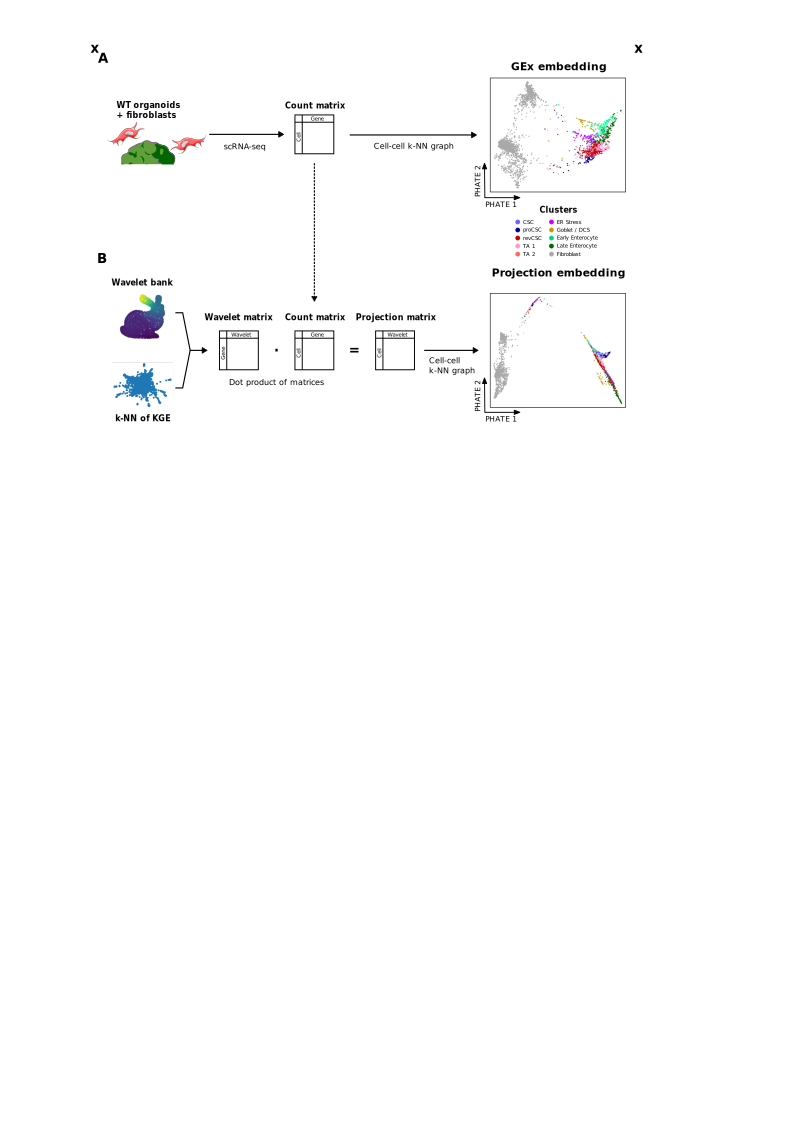
\includegraphics{06kg/figs/6KG_projection.png}
    \caption{}
    \label{fig:6project}
\end{figure}

Organoid dataset. Wt stromal coculture where fibs talk to WT epi cells (Figure \ref{fig:4cc}A). Embed count matrix reveals 2 cells types and epithelial heterogeneity.

Given the KGE, generate a \emph{k}-NN graph onto which I apply a wavelet bank on nodes at series of scales. This difussion process generates a wavelet matrix onto which the gene expression matrix can be projected.

Leveraging the properties of the dot product (\(\cdot\)) operation between matrices, I compute the product between the \(node X wavelets\) matrix and the \(cell X feature\) count matrix, where the features are formatted as gene symbols like in the \acrshort{kg}. This results in a new projected matrix of \(cell X wavelets\) dimensions (Figure \ref{}).

Resulting projection topologically resembles GEx data on PHATE embedding, albeit it appears there is some signal loss as epithelial heterogeneity is not as noticeable.

\begin{figure}
    \centering
    \includegraphics{06kg/figs/6KG_bench.png}
    \caption{}
    \label{fig:6bench}
\end{figure}

Porjection results can be assed quantitaively by comparing cell-cell distance between the GEx graph and projected graph. given what we know on fibs interacting with revCSC and TA 2, wee would expectd thos differences to be decreased on projected space.

We thus construcut 2 knn, from gex and from LRT projection, and then compute the median/average distance between clusters. To compare two distance datasets, relative values established.

Mixed results tbh.

\newpage
\section{Conclusions}

\colorbox{yellow}{OUTLINE (WIP)}
* Built LRT KG that is comparable to other directed graphs in literature.
    * IF omnpath capture ground bio truth, cell commns are indeed mostly hierarhcical. WE have a simplified hyper hierarhcical version.
* KG embedding methods seem to conserve biological properties associted with nodes.
* Wavelets used to difusse signal on graph so that single-cell \emph{omic} data can be projected on it.
* Results match/conserve broader GEx information, but information gain is limited regarding cell communications.
* Need to improve signal difussion step. Alternative gene embedding step can also be explored (GSP paper), so can the benchmarking be improved.

Fine balance between signal loss determined by lmited number of gene nodes on graph, but also on graph structure itself being important enough to produce results signficantly different from GEx matrix.